\documentclass[tikz,border=8pt]{standalone}
\usepackage{amsmath}
\usetikzlibrary{arrows.meta}
\definecolor{ink}{HTML}{21352F}
\definecolor{teal}{HTML}{087F7B}
\definecolor{blue}{HTML}{4B77A8}
\definecolor{gold}{HTML}{C58B2A}
\definecolor{rose}{HTML}{B65A62}
\begin{document}
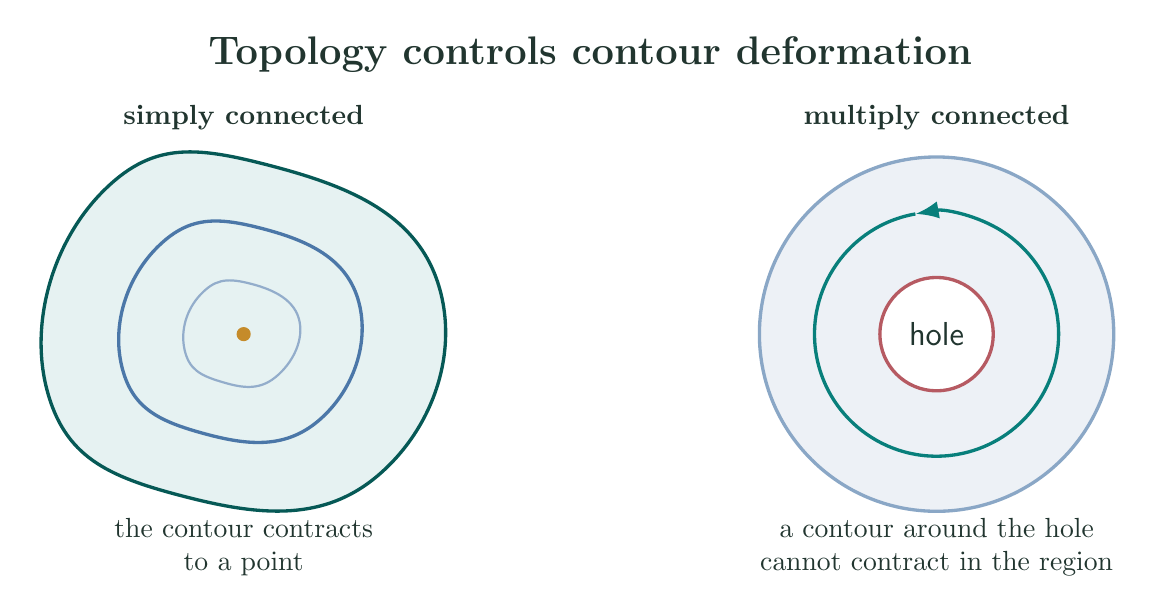
\begin{tikzpicture}[font=\large\sffamily,text=ink,>=Latex]
  \node[font=\bfseries\Large] at (0,3.55)
    {Topology controls contour deformation};

  \begin{scope}[xshift=-4.4cm]
    \node[font=\bfseries] at (0,2.75) {simply connected};
    \path[fill=teal!10,draw=teal!70!black,very thick]
      plot[smooth cycle,tension=.8] coordinates
      {(-2.5,-.7)(-1.8,1.8)(.3,2.15)(2.45,.7)(1.7,-1.8)(-.8,-2.05)};
    \draw[blue,very thick,->]
      plot[smooth cycle,tension=.8] coordinates
      {(-1.55,-.4)(-1.1,1.1)(.2,1.35)(1.45,.45)(.95,-1.1)(-.55,-1.25)};
    \draw[blue!60,thick,->]
      plot[smooth cycle,tension=.8] coordinates
      {(-.75,-.2)(-.55,.5)(.05,.65)(.7,.2)(.4,-.55)(-.3,-.6)};
    \fill[gold] (0,0) circle (.09);
    \node[font=\normalsize,align=center] at (0,-2.7)
      {the contour contracts\\to a point};
  \end{scope}

  \begin{scope}[xshift=4.4cm]
    \node[font=\bfseries] at (0,2.75) {multiply connected};
    \fill[blue!10] (0,0) circle (2.25);
    \draw[blue!65,very thick] (0,0) circle (2.25);
    \fill[white] (0,0) circle (.72);
    \draw[rose,very thick] (0,0) circle (.72);
    \draw[teal,very thick,->] (1.55,0)
      arc[start angle=0,end angle=100,radius=1.55];
    \draw[teal,very thick] ({1.55*cos(100)},{1.55*sin(100)})
      arc[start angle=100,end angle=360,radius=1.55];
    \node at (0,0) {hole};
    \node[font=\normalsize,align=center] at (0,-2.7)
      {a contour around the hole\\cannot contract in the region};
  \end{scope}
\end{tikzpicture}
\end{document}
